\documentclass[a4paper,11pt,twocolumn]{article}
\usepackage{fancyhdr}
\usepackage{enumerate}
\usepackage{times}
\usepackage{mathptmx}
\usepackage{amsmath}
\usepackage{amsfonts}
\usepackage{amssymb}
\usepackage{tikz}
\usepackage[top=2cm, bottom=2cm, left=2cm, right=2cm]{geometry}

\setlength{\columnsep}{7mm}

\newcommand{\homeworkno}{3.5}
\pagestyle{fancy}
\lhead{Problem Solving: Homework \homeworkno}
\chead{}
\rhead{Chen Shaoyuan (161240004)}
\lfoot{}
\cfoot{\thepage}
\rfoot{}

\allowdisplaybreaks[4]
\renewcommand{\labelenumi}{\textbf{\emph{\alph{enumi}}.}}
\begin{document}
  \title{Problem Solving: Homework \homeworkno}
  \author{Name: Chen Shaoyuan \and Student ID: 161240004}
  \maketitle

  \section{[GC] Problem 26.1-1}
  For every feasible flow $f$ in $G'$, by flow conservation and capacity constraint, $f(u, x) = f(x, v) \leq c(x, v)$. If we define $f': V(G) \times V(G) \rightarrow \mathbb{R}$:
  $$ f'(a, b) = \begin{cases} f(u, x) & a = u, b = y \\ f(a, b) & \text{otherwise} \end{cases}, $$
  $f'$ is still a feasible flow of $G$ with equal value because it still satisfies capacity constraint and flow conservation, and the total flow out of the source do not change. Likewise, for every feasible flow in $G$, we can find out a corresponding flow in $G'$ with equal value. Therefore, a maximum flow in $G'$ has the same value as a maximum flow in $G$.

  \section{[GC] Problem 26.1-2}
  Let $G$ denote the flow network with multiple sources and multiple sinks, and $G'$ denote the corresponding single-source, single-sink flow network. For every feasible flow $f$ in $G$, we define $f': V(G') \times V(G') \rightarrow \mathbb{R}$:
  $$ f'(a, b) = \begin{cases} \sum\limits_{x}f(b, x) & a = s' \\ \sum\limits_{x} f(x, a) & b = t' \\ f(a, b) & \text{otherwise} \end{cases}, $$
  where $s'$ is the supersource and $t'$ is the supersink, we can easily verify that $f'$ is  a feasible flow of $G'$ with equal value. \par
  For every feasible flow $f'$ in $G'$, if we simply define a flow $f$ of $G$ as $f(a, b) = f'(a, b)$ for all $a, b \in V(G)$, we get a feasible flow of $G$ with the same value as $f'$.

  \section{[GC] Problem 26.1-6}
  First, model the map of the town as a symmetric directed graph. Then, assign capacity 1 to each arc in the graph. Finally, let their home be the source, and the school be the sink, and compute the max-flow of the flow network. It is possible that both his children can go to the same school if and only if the max-flow is not less than 2.

  \section{[GC] Problem 26.1-7}
  We replace each vertex $v$ in $V$ by $v_i$ and $v_o$, and replace each edge $(u, v)$ by $(u_o, v_i)$, with the capacity unchanged. Then we add an edge $(v_i, v_o)$ for each $v$ with capacity $l(v)$. The maximum flow of the new network is the same as the original one with vertex capacities. In the new graph, there are $2|V|$ vertices and $|V|+|E|$ edges.

  \section{[GC] Problem 26.2-2}
  The flow across the cut is 19, and the capacity of the cut is 31.

  \section{[GC] Problem 26.2-6}
  We add a supersource $s$ and a supersink $t$ to this network, and edges $(s, s_i)$ with capacities $p_i$, $(t_j, t)$ with capacities $q_j$. Then compute the maximum flow $f$ of the new network. The flow obeying these constrains in multiple-source multiple-sink flow network exists if and only if the flow $f$ we find obeys these constrains. Otherwise, there must exist an augmenting path from some source to some sink without violating the constrains, and the flow we find before is not a maximum flow.

  \section{[GC] Problem 26.2-8}
  The Ford-Fulkerson method repeatedly finds an augmenting path from $s$ to $t$, and add it to current flow. Note that a path from $s$ to $t$ never contains an edge to $s$. Therefore, the procedure still correctly computes a maximum flow.

  \section{[GC] Problem 26.2-10}
  Assume that we have already found a maximum flow $f$. Let $(u, v)$ be the edge such that $f(u, v)$ has minimum positive value. Then find a path containing this edge from $s$ to $t$. Since for every edge $e$ in the path, the flow passing through $e$ is at least $f(u, v)$, we decrease the flows of these edges by $f(u, v)$; furthermore, we can remove edge $(u, v)$. Repeatedly doing this will finally decompose the flow into at most $|E|$ augmenting paths.

  \section{[GC] Problem 26.2-12}
  By flow conservation property, there must exist a cycle, or a path from $t$ to $s$, containing $(v, s)$. Decreasing the flow of each edge in the cycle or path by 1 yields another maximum flow $f'$ with $f'(v, s) = 0$. To find such cycle or path, we only have to perform DFS or BFS on $f$ from the edge $(v, s)$, which takes $O(E)$ time.

  \section{[GC] Problem 26.2-12}
  For every edge $(u, v)$, we change its capacity from $c(u, v)$ to $c(u, v)(|E|+1)+1$. If the minimum cut of the new network is $c(S, T)$, then the minimum cut of the original network is $\lfloor c(S, T) / (|E|+1) \rfloor$, which contains $c(S, T) \bmod (|E|+1)$ edges.

  \section{[GC] Problem 26.3-3}
  The length of any augmenting path is at most $|V|-1$, because every vertex appears in the path at most once. We can show that the bound is sharp: consider graph $P_{2n}$ (a graph of order $2n$ which only contains a chain), it is bipartite and the length of the only augmenting path is $2n-1$.

  \section{[GC] Problem 26-1}
  \begin{enumerate}
    \item See Problem 26.1-7.
    \item We model this grid as a flow network, for every vertex and edge in which, we assign unit capacity. We treat the $m$ points to escape as sources, and the points in the boundary as sinks. Now the escape problem has been reduced to multi-source multi-sink maximum flow problem, with vertex capacities allowed. If we choose Ford-Fulkerson method as max-flow algorithm, the total running time is $O(mn^2)$. Note that there are only $4n-4$ sinks, so if $m > 4n-4$, the grid does not have an escape. So the running time can be optimized to $O(\min(n, m)n^2)$.
  \end{enumerate}

  \section{[GC] Problem 26-2}
  \begin{enumerate}
    \item For every vertex $v$ in the original graph, we split it into two vertices $v_i$, $v_o$ in the new graph, and for every arc $(u, v)$ in the original graph, we add edge $(u_o, v_i)$ into the new graph. The new graph is bipartite, and we compute a maximum bipartite matching on the new graph. For every matched vertices in the maximum bipartite matching, we join the corresponding vertices in the original graph, forming a longer path. Finally, we will get a maximum path cover.
    \item No. Consider the following graph and its minimum path cover
    \small
    \begin{center}
    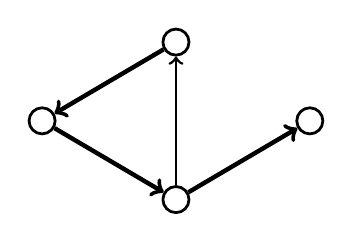
\begin{tikzpicture}[line width = 1pt,
                        solid/.style = {circle, draw, fill = black, minimum size = 0.1cm},
                        empty/.style = {circle, draw, fill = white, minimum size = 0.1cm}]
      \node [empty] (a1) at (0, 0){};
      \node [empty] (a2) at (1.7, 1){};
      \node [empty] (a3) at (1.7, -1){};
      \node [empty] (a4) at (3.4, 0){};
      \draw [->, ultra thick] (a1) -- (a3);
      \draw [->] (a3) -- (a2);
      \draw [->, ultra thick] (a2) -- (a1);
      \draw [->, ultra thick] (a3) -- (a4);
    \end{tikzpicture}
    \end{center} \par
    \normalsize
    If we compute the maximum matching of the derived bipartite graph, one possible maximum matching is 
    \small
    \begin{center}
    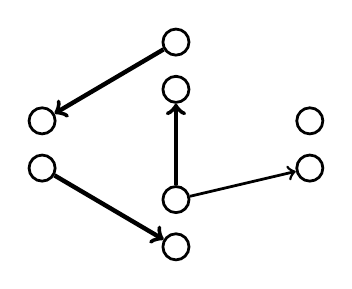
\begin{tikzpicture}[line width = 1pt,
                        solid/.style = {circle, draw, fill = black, minimum size = 0.1cm},
                        empty/.style = {circle, draw, fill = white, minimum size = 0.1cm}]
      \node [empty] (a1) at (0, 0.3){};
      \node [empty] (b1) at (0, -0.3){};
      \node [empty] (a2) at (1.7, 1.3){};
      \node [empty] (b2) at (1.7, 0.7){};
      \node [empty] (a3) at (1.7, -0.7){};
      \node [empty] (b3) at (1.7, -1.3){};
      \node [empty] (a4) at (3.4, 0.3){};
      \node [empty] (b4) at (3.4, -0.3){};
      \draw [->, ultra thick] (b1) -- (b3);
      \draw [->, ultra thick] (a2) -- (a1);
      \draw [->, ultra thick] (a3) -- (b2);
      \draw [->] (a3) -- (b4);
    \end{tikzpicture}
    \end{center} \par
    \normalsize
    according this matching, the original graph can be covered by a cycle and an isolated vertex, which is not minimum.
  \end{enumerate}
\end{document}
